\documentclass[10pt]{beamer}
\usepackage[utf8]{inputenc}
\usepackage[T1]{fontenc}
\usepackage{graphicx}
\usepackage{amssymb}
\usepackage{booktabs}
\usepackage{array}
\newcolumntype{L}[1]{>{\raggedright\arraybackslash}p{#1}}
\usetheme{CambridgeUS}
\usecolortheme{dolphin}
\usepackage{tikz}
\usetikzlibrary{arrows.meta, positioning}
\definecolor{myNewColorA}{RGB}{126,12,110}
\definecolor{myNewColorB}{RGB}{165,85,154}
\definecolor{myNewColorC}{RGB}{203,158,197}
\setbeamercolor*{palette primary}{bg=myNewColorC}
\setbeamercolor*{palette secondary}{bg=myNewColorB, fg=white}
\setbeamercolor*{palette tertiary}{bg=myNewColorA, fg=white}
\setbeamercolor*{titlelike}{fg=myNewColorA}
\setbeamercolor*{title}{bg=myNewColorA, fg=white}
\setbeamercolor*{item}{fg=myNewColorA}
\setbeamercolor*{caption name}{fg=myNewColorA}
\setbeamercolor*{block title}{bg=myNewColorB, fg=white}
\setbeamercolor*{block body}{bg=myNewColorC!25}
\setbeamercolor*{block title example}{bg=orange!75!black, fg=white}
\setbeamercolor*{block body example}{bg=orange!12}
\usefonttheme{professionalfonts}
\setbeamertemplate{caption}[numbered]
\newcommand{\highlight}[1]{\textcolor{myNewColorA}{\textbf{#1}}}

% ---- running example: a cat on a sofa, cut into 6x6 = 36 patches (toy size) ----
\colorlet{catc}{orange!85}
\colorlet{bgc}{teal!25}
\colorlet{keptc}{teal!55}
\colorlet{dropc}{black!85}
% #1 cat fill, #2 background fill, #3 list of special background cells (x/y), #4 their fill, #5 cell size
\newcommand{\catgrid}[5]{%
\begin{tikzpicture}[x=#5,y=#5]
\foreach \gx in {0,...,5}{\foreach \gy in {0,...,5}{\filldraw[fill=#2, draw=white, line width=0.4pt] (\gx,\gy) rectangle ++(1,1);}}
\foreach \gx/\gy in {#3}{\filldraw[fill=#4, draw=white, line width=0.4pt] (\gx,\gy) rectangle ++(1,1);}
\foreach \gx/\gy in {2/3,3/3,1/2,2/2,3/2,4/2,1/1,2/1}{\filldraw[fill=#1, draw=white, line width=0.4pt] (\gx,\gy) rectangle ++(1,1);}
\end{tikzpicture}}
% real photo (img/cat.jpg) with the 6x6 patch grid; the 8 cat patches are tinted orange (same cells as \catgrid)
\newcommand{\catphoto}[1]{%
\begin{tikzpicture}[x=#1,y=#1]
\node[anchor=south west, inner sep=0] at (0,0) {\includegraphics[width=6\dimexpr#1\relax]{img/cat.jpg}};
\foreach \gx/\gy in {2/3,3/3,1/2,2/2,3/2,4/2,1/1,2/1}{\fill[orange, opacity=0.35] (\gx,\gy) rectangle ++(1,1);}
\foreach \gx in {0,...,5}{\foreach \gy in {0,...,5}{\draw[white, line width=0.5pt] (\gx,\gy) rectangle ++(1,1);}}
\foreach \gx/\gy in {2/3,3/3,1/2,2/2,3/2,4/2,1/1,2/1}{\draw[orange!90!black, line width=0.9pt] (\gx,\gy) rectangle ++(1,1);}
\end{tikzpicture}}
% grid + caption, small version
\newcommand{\catpic}[5]{\begin{minipage}[t]{2.15cm}\centering\catgrid{#1}{#2}{#3}{#4}{0.32cm}\\[2pt]{\tiny #5}\end{minipage}}
% orange example box
\newcommand{\catex}[1]{\begin{exampleblock}{\footnotesize Cat example (illustration, not from the paper)}\footnotesize #1\end{exampleblock}}

\setbeamerfont{title}{size=\large}
\setbeamerfont{subtitle}{size=\small}
\setbeamerfont{author}{size=\small}
\setbeamerfont{institute}{size=\small}
\setbeamerfont{block title}{size=\small}
\setbeamerfont{block body}{size=\small}

\title[XAI for ViTs: Sections 3.4--8]{\textbf{EXPLAINABILITY OF VISION TRANSFORMERS}}
\subtitle{\textbf{Inherently Explainable and Task-specific Methods,\\ Evaluation, Tools and Outlook}\\[2pt]
\scriptsize Sections 3.4--8 of Kashefi et al., \emph{Explainability of Vision Transformers: A Comprehensive Review and New Perspectives} (arXiv:2311.06786, 2023)}
\author[Group 6]{[Your name] \and [Teammates]}
\institute[Group 6]{University of Science - VNUHCM}
\date{}

\begin{document}

\frame{\titlepage}

%============================================================
% DEMO for Section 3.2 (Attention-based methods): reproduction of Fig. 3 of the survey
%============================================================
\section{Demo 3.2 Attention-based methods}

\begin{frame}{Demo for 3.2 Attention-based Methods: what we did}
\begin{itemize}\small
  \item \textbf{Goal:} re-run the experiment behind \highlight{Fig.~3 of the survey} (class-specific visualizations, Chefer et al., 2021a) and check its claims ourselves.
  \item \textbf{Model:} ViT-B/16 pretrained on ImageNet. \textbf{Code:} the authors' official repository \texttt{Transformer-Explainability}.
  \item \textbf{Inputs:} 2 photos $\times$ 2 classes = 4 rows. We ask the model about \emph{each} class separately.
\end{itemize}
\vspace{0.1em}
\begin{center}\footnotesize
\begin{tabular}{L{2.8cm}L{3.8cm}L{1.6cm}}
\toprule
\textbf{Photo} & \textbf{Class we explain} & \textbf{Class id}\\
\midrule
dog + cat & Dog (bull mastiff), Cat & 243, 282\\
elephant + zebra & Elephant (tusker), Zebra & 101, 340\\
\bottomrule
\end{tabular}
\end{center}
\begin{block}{Pipeline for every row}
\footnotesize
\begin{enumerate}
  \item Resize the photo to $224\times224$ and normalize.
  \item Forward pass: the model gives one score per class.
  \item Pick class $c$, then \textbf{backward pass} (gradients / LRP relevance).
  \item Get one number per patch: a $14\times14$ map.
  \item Upsample $\times16$, min--max normalize, overlay as a heat map.
\end{enumerate}
\end{block}
\end{frame}

\begin{frame}{Six columns, six answers to ``which patches matter?''}
\footnotesize
\begin{tabular}{L{2.1cm}L{5.9cm}L{1.9cm}}
\toprule
\textbf{Method} & \textbf{What the official code computes} & \textbf{Class-specific?}\\
\midrule
rollout & Multiply the attention matrices of all 12 layers (identity added for the skip connection); read the class-token row & No\\[2pt]
raw-attention & Attention from the class token to the patches in the \textbf{last layer}, averaged over heads & No\\[2pt]
GradCAM & Last-layer attention map $\times$ its gradient with respect to the class score & Yes\\[2pt]
LRP & Relevance of the class score propagated back \textbf{all the way to the pixels} & Yes (by design)\\[2pt]
partial LRP & LRP relevance of the \textbf{last attention layer only} & Partly\\[2pt]
\highlight{Beyond Attention} & \textbf{Every layer:} positive part of (gradient $\times$ LRP relevance of attention), averaged over heads, then chained like rollout & Yes\\
\bottomrule
\end{tabular}
\vspace{0.3em}
\catex{Same dog-and-cat photo. Class-agnostic methods give one map for ``dog'' and ``cat'': they only show where the model looks. A class-specific method gives a different map for each question.}
\end{frame}

\begin{frame}{Our reproduction of Fig.~3}
\centering
\includegraphics[width=0.94\textwidth]{img/demo_ours_fig3.png}\\[2pt]
{\tiny Rows: class asked. Columns: method. Red = most important patches.}
\end{frame}

\begin{frame}{Does it match the paper?}
\begin{columns}[T]
\column{0.44\textwidth}
\centering
\includegraphics[width=\textwidth]{img/paper_fig3.png}\\[1pt]
{\tiny Fig.~3 in the survey (Kashefi et al., 2023)}\\[4pt]
\includegraphics[width=\textwidth]{img/demo_ours_fig3.png}\\[1pt]
{\tiny Our run}
\column{0.54\textwidth}
\footnotesize
\begin{itemize}
  \item[\checkmark] \textbf{rollout, raw-attention:} same map for both classes.
  \item[\checkmark] \textbf{LRP:} noisy, washed-out, little class information.
  \item[\checkmark] \textbf{Beyond Attention:} cleanest; follows the class (dog head vs.\ cat, zebra vs.\ elephant).
  \item[\checkmark] Model prediction as in the authors' notebook: top-1 = cat (52\%) and zebra (74\%).
  \item[$\approx$] Not pixel-identical: we resize the whole photo to $224\times224$; the paper may crop differently.
\end{itemize}
\begin{block}{Conclusion}
\footnotesize The qualitative claims of the paper are \textbf{reproduced}: only the class-specific methods separate the two classes, and Beyond Attention does it best.
\end{block}
\end{columns}
\end{frame}

\begin{frame}{Outline of this part}
\begin{columns}[T]
\column{0.52\textwidth}
\begin{enumerate}
  \item[\textbf{3.4}] Inherently explainable methods
  \item[\textbf{3.5}] Explainability of other tasks
  \item[\textbf{4}] Explanation evaluation
  \item[\textbf{5--6}] Tools and datasets
  \item[\textbf{7--8}] Discussion and conclusion
\end{enumerate}
\column{0.46\textwidth}
\centering
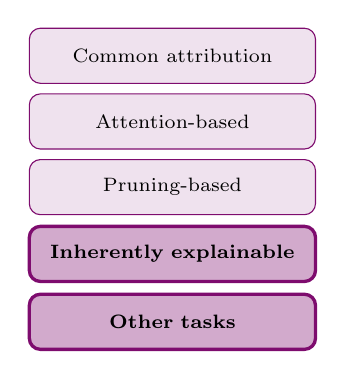
\begin{tikzpicture}[font=\scriptsize,
  b/.style={draw=myNewColorA, fill=myNewColorC!30, rounded corners, align=center, minimum height=0.7cm, text width=3.4cm}]
  \node[b] (a) {Common attribution};
  \node[b, below=0.12cm of a] (b1) {Attention-based};
  \node[b, below=0.12cm of b1] (c) {Pruning-based};
  \node[b, below=0.12cm of c, fill=myNewColorA!35, line width=1.2pt] (d) {\textbf{Inherently explainable}};
  \node[b, below=0.12cm of d, fill=myNewColorA!35, line width=1.2pt] (e) {\textbf{Other tasks}};
\end{tikzpicture}\\[2pt]
{\scriptsize Taxonomy of the survey (Fig.~2): bold = this part}
\end{columns}
\end{frame}

%============================================================
\begin{frame}{Running example: a cat on a sofa}
\begin{columns}[T]
\column{0.42\textwidth}
\centering
\catphoto{0.7cm}\\[3pt]
{\scriptsize Photo cut into $6\times6=36$ patches\\ {\color{orange!85!black}\textbf{8 cat patches}} (orange) \;+\; \textbf{28 sofa patches}}\\[1pt]
{\tiny Photo: Kafun, CC BY-SA 4.0, Wikimedia Commons}
\column{0.56\textwidth}
\begin{itemize}
  \item The ViT looks at this photo and answers: \highlight{``cat''}.
  \item \textbf{The question of the whole talk:} \emph{which patches did the model really need to say ``cat''?}
  \item Every method in this part is a different way to answer this question.
\end{itemize}
\vspace{0.3em}
\catex{Real ViTs usually cut a $224\times224$ photo into $14\times14=196$ patches. We use 36 only to keep the drawings small.}
\end{columns}
\end{frame}

\begin{frame}{Key terms you need (full glossary in the script)}
\small
\begin{tabular}{L{2.5cm}L{4.4cm}L{3.5cm}}
\toprule
\textbf{Term} & \textbf{Meaning} & \textbf{Cat example}\\
\midrule
Patch / token & A small square piece of the image, treated like a ``word'' by the transformer & 1 of the 36 squares\\[2pt]
Class token & A special extra token that collects information from all tokens and gives the final answer & The ``team leader'' that says ``cat''\\[2pt]
Attention & How much one token ``looks at'' another token (a number) & Cat-ear patch looks strongly at cat-face patch\\[2pt]
Saliency map & A heat map showing how important each patch is for the answer & Bright on the cat, dark on the sofa\\[2pt]
Faithful vs.\ plausible & Faithful = matches what the \emph{model} really uses. Plausible = looks reasonable to \emph{humans}. & Model may use the sofa; a human expects the cat\\
\bottomrule
\end{tabular}
\end{frame}

%============================================================
\section{3.4 Inherently explainable methods}

\begin{frame}{3.4 Inherently Explainable Methods and ViT-CX}
\begin{itemize}\small
  \item Approaches that develop models able to \highlight{explain themselves}.
  \item They may use interpretable tools such as \textbf{decision trees} or \textbf{rule-based systems}, or \textbf{enforce sparsity}.
  \item But they often \textbf{struggle to reach the accuracy of black-box models}: balance needed (Rudin, 2019).
\end{itemize}
\begin{block}{ViT-CX (Xie et al., 2022)}
\begin{itemize}\small
\item A \textbf{mask-based} explanation method customized for ViT.
\item Relies on \textbf{patch embeddings} and their \textbf{causal impact on the output}, not on the attention given to them.
\item Two phases: \textbf{mask generation} and \textbf{mask aggregation}.
\item More meaningful saliency maps, \textbf{significantly better faithfulness}.
\end{itemize}
\end{block}
\catex{Make many masks that hide different parts of the photo. Masks that keep the cat face leave the score ``cat'' high; masks that hide it make the score fall. Combine all masks, weighted by their effect, into one heat map.}
\end{frame}

\begin{frame}{Patch Interactions (Ma et al., 2023) and ViT-NeT (Kim et al., 2022)}
\begin{columns}[T]
\column{0.5\textwidth}
\textbf{Visualizing patch-wise interactions}
\begin{itemize}\small
  \item \textbf{Quantify} patch-wise interaction, then \textbf{identify indiscriminative patches}.
  \item \highlight{Adaptive attention window} constrains each patch's receptive field.
  \item \textbf{Main-object patches} have \textbf{smaller} receptive fields than background patches.
  \item Small fields learn \textbf{local textures / structures}; large fields learn the \textbf{object--background correlation}.
\end{itemize}
\column{0.5\textwidth}
\textbf{ViT-NeT}
\begin{itemize}\small
  \item A ViT with a \highlight{neural tree decoder}.
  \item Describes decisions through a \textbf{tree structure and prototypes}.
  \item Enables \textbf{visual interpretation}.
  \item Good for \textbf{fine-grained} classification: similarities \textbf{between classes} and variations \textbf{within a class}.
\end{itemize}
\end{columns}
\vspace{0.2em}
\catex{\textbf{Patch interactions}: a cat patch only looks at neighbours to learn fur texture (small field); a sofa patch looks far, linking cat and background (large field). \textbf{ViT-NeT}: like 20 questions -- ``pointed ears? whiskers?'' $\to$ ``Siamese cat, this patch matches the stored ear prototype''.}
\end{frame}

\begin{frame}{R-Cut (Niu et al., 2023)}
\textbf{R-Cut}: enhancing explainability with \highlight{Relationship Weighted Out and Cut}.
\vspace{0.4em}
\begin{columns}[T]
\column{0.48\textwidth}
\begin{block}{Relationship Weighted Out}
Extracts \textbf{class-specific information} from intermediate layers and \textbf{emphasizes relevant features}.
\end{block}
\column{0.48\textwidth}
\begin{block}{Cut}
Performs \textbf{fine-grained feature decomposition}, taking \textbf{position, texture and color} into account.
\end{block}
\end{columns}
\vspace{0.4em}
\begin{itemize}
  \item Integrating the two modules yields \textbf{dense, class-specific visual explainability maps}.
  \item Evaluated with the \textbf{IoU test} (Section 4).
\end{itemize}
\catex{Step 1: pull out what the middle layers know about ``cat''. Step 2: split the picture into groups by position, texture and colour (head, body, sofa). Result: a detailed heat map that lights up the cat.}
\end{frame}

%============================================================
\section{3.5 Other tasks}

\begin{frame}{3.5 Explainability of Other Tasks: eX-ViT and DINO}
Explainability of ViT beyond classification is \textbf{still being explored}; early results are promising.
\vspace{0.3em}
\begin{columns}[T]
\column{0.5\textwidth}
\begin{block}{eX-ViT (Yu et al., 2023)}
\scriptsize
\begin{itemize}
\item For \textbf{weakly supervised semantic segmentation}.
\item \textbf{Siamese network}: two branches process two augmented versions of an input, self-supervised.
\item Each branch: \textbf{Explainable Multi-Head Attention} and \textbf{Attribute-guided Explainer}.
\item Three losses: \textbf{global-level attribute-guided}, \textbf{local-level attribute discriminability}, \textbf{attribute diversity}.
\end{itemize}
\end{block}
\column{0.5\textwidth}
\begin{block}{DINO (Caron et al., 2021)}
\scriptsize
\begin{itemize}
\item A simple \textbf{self-supervised} method: \textbf{self-distillation with no labels}.
\item Learned \textbf{attention maps preserve the semantic regions} of images.
\item These maps can be used \textbf{for explanation}.
\end{itemize}
\end{block}
\end{columns}
\catex{\textbf{eX-ViT}: we only know ``this photo has a cat'' but want its outline; a flipped and a darker copy of the photo must give consistent maps. \textbf{DINO}: no labels at all, yet attention already covers the cat.}
\end{frame}

\begin{frame}{Generic Attention-model, ATMAN, Concept-Transformer}
\footnotesize
\begin{block}{Generic Attention-model (Chefer et al., 2021b)}
Explains \textbf{bi-modal transformers} and those with \textbf{co-attention}; three architectures: \textbf{pure self-attention}, \textbf{self- + co-attention}, \textbf{encoder-decoder attention}. Tested on \textbf{visual question answering}; also applicable to detection and segmentation.
\end{block}
\begin{block}{ATMAN (Deb et al., 2023)}
A \textbf{modality-agnostic perturbation method} that \textbf{manipulates attention} (memory-efficient) to produce \textbf{relevance maps} of the input w.r.t.\ the output.
\end{block}
\begin{block}{Concept-Transformer (Rigotti et al., 2022)}
Generalizes attention from \textbf{low-level features} to \textbf{high-level, user-defined concepts}; explanations are \textbf{attention scores over concepts}, ensuring \textbf{plausibility and faithfulness}.
\end{block}
\catex{\textbf{Generic}: photo + question ``What is on the sofa?'' $\to$ shows which words \emph{and} which patches led to ``cat''. \textbf{ATMAN}: weaken the attention paid to the face patches \emph{inside} the model and see how much the answer changes. \textbf{Concept-Transformer}: ``pointed ears 0.8, whiskers 0.7, fur 0.6'' instead of pixels.}
\end{frame}

%============================================================
\section{4 Explanation evaluation}

\begin{frame}{4 Explanation Evaluation}
\begin{itemize}
  \item Assessing how well a method depicts a model's reasoning is \textbf{challenging}.
  \item The literature suggests \textbf{evaluative criteria} (Fig.~5 of the survey).
\end{itemize}
\vspace{0.2em}
\centering
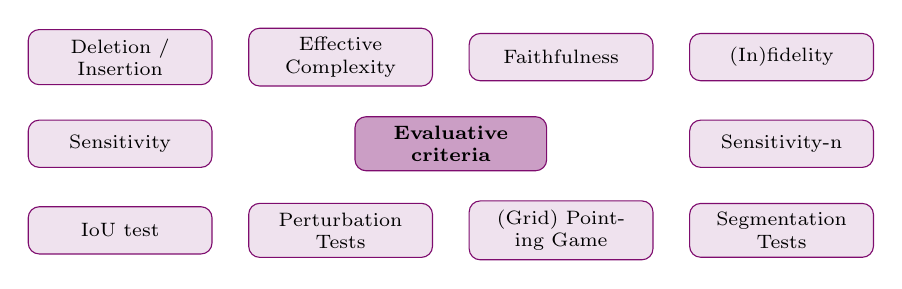
\begin{tikzpicture}[font=\scriptsize, every node/.style={draw=myNewColorA, fill=myNewColorC!30, rounded corners, align=center, minimum height=0.6cm, text width=2.1cm}]
 \node[fill=myNewColorA!40, text width=2.2cm] (c) at (0,0) {\textbf{Evaluative criteria}};
 \node (a1) at (-4.2,1.1) {Deletion / Insertion};
 \node (a2) at (-1.4,1.1) {Effective Complexity};
 \node (a3) at (1.4,1.1) {Faithfulness};
 \node (a4) at (4.2,1.1) {(In)fidelity};
 \node (b1) at (-4.2,-1.1) {IoU test};
 \node (b2) at (-1.4,-1.1) {Perturbation Tests};
 \node (b3) at (1.4,-1.1) {(Grid) Pointing Game};
 \node (b4) at (4.2,-1.1) {Segmentation Tests};
 \node (d1) at (-4.2,0) {Sensitivity};
 \node (d2) at (4.2,0) {Sensitivity-n};
\end{tikzpicture}
\vspace{0.3em}
\begin{flushleft}\catex{We have a heat map that says ``the cat is why''. \emph{How do we know the heat map is right?} Each criterion below checks it in a different way.}\end{flushleft}
\end{frame}

\begin{frame}{Deletion / Insertion and Perturbation Tests}
\footnotesize
\begin{block}{Deletion and Insertion (Petsiuk et al., 2018)}
Evaluate the \textbf{faithfulness} of a saliency map to the model.
\begin{itemize}\footnotesize
\item \textbf{Deletion AUC}: how quickly the class score \textbf{declines} when important pixels are \textbf{omitted}.
\item \textbf{Insertion AUC}: how quickly the class score \textbf{increases} when important pixels are \textbf{added to a blank canvas}.
\item \textbf{Smaller Deletion AUC, larger Insertion AUC} = higher faithfulness.
\end{itemize}
\end{block}
\begin{block}{Perturbation tests}
Gradually \textbf{mask input tokens} following the explanation; accuracy summarized by the \textbf{AUC}.
\begin{itemize}\footnotesize
\item \textbf{Positive}: mask from \emph{most} to \emph{least} relevant; \textbf{sharp drop} expected.
\item \textbf{Negative}: mask from \emph{least} to \emph{most} relevant; a good explanation \textbf{preserves accuracy}.
\end{itemize}
\end{block}
\catex{Score(cat) = 0.95. \textbf{Good map} (cat first): deleting the 8 cat patches gives 0.10 $\Rightarrow$ small Deletion AUC. \textbf{Bad map} (sofa first): still 0.93 $\Rightarrow$ large AUC. Insertion = mirror: adding cat patches first to a blank canvas lifts the score to 0.90.}
\end{frame}

\begin{frame}{Effective Complexity, Faithfulness and (In)fidelity}
\scriptsize
\begin{block}{Effective Complexity}
Counts the \textbf{number of attributions above a threshold}. Low value: some features can be ignored $\Rightarrow$ \textbf{simpler, more integrated explanation}, at some cost of factual accuracy.
\end{block}
\begin{block}{Faithfulness}
Assesses attributions \textbf{without human intervention}: removes features and analyzes the \textbf{linear correlation} between the predicted logits and the attribution of the removed subset. Several runs/samples; value in \textbf{$[-1,1]$}.
\end{block}
\begin{block}{(In)fidelity}
How well an explanation \textbf{captures changes in the prediction} under significant input perturbations. \textbf{Minimize} it: low infidelity = \textbf{high-fidelity explanation}. Complementary to sensitivity.
\end{block}
\catex{\textbf{EC}: 36 map values, only 8 above the threshold $\Rightarrow$ EC = 8 (clean). \textbf{Faithfulness}: remove random groups of patches; the bigger the map's value for a group, the more the score should fall (correlation near $+1$). \textbf{Infidelity}: add strong noise; the map should predict the fall.}
\end{frame}

\begin{frame}{Sensitivity and Sensitivity-$n$}
\begin{block}{Sensitivity}
Assesses \textbf{how explanations vary with minor input perturbations}. Similar inputs with close outputs $\Rightarrow$ \textbf{similar explanations}.
\end{block}
\begin{block}{Sensitivity-$n$}
Tests the \textbf{attribution values}, not only the ranking.
\begin{itemize}\small
\item Randomly selects \textbf{subsets of $n$ features}.
\item \textbf{Correlation} between the \textbf{change of the prediction} when they are removed and the \textbf{sum of their attribution scores}.
\item Averaged over many subsets. \textbf{High score} = accurate attributions.
\end{itemize}
\end{block}
\catex{\textbf{Sensitivity}: two photos of the same cat, differing by invisible noise, both say ``cat'' $\Rightarrow$ their maps must look the same. \textbf{Sensitivity-$n$} ($n=5$): remove 5 random patches; the score falls by 0.30; the map's values for those 5 patches sum to 0.28 $\Rightarrow$ close. Repeat for many subsets and check the correlation.}
\end{frame}

\begin{frame}{IoU, Pointing Game and Segmentation Tests}
\footnotesize
\begin{columns}[T]
\column{0.5\textwidth}
\textbf{IoU test}
\begin{itemize}
\item Overlap of the explanation with the \textbf{ground-truth bounding box}.
\item Upsample map to image size, \textbf{threshold 0.2} to drop background.
\item IoU = \textbf{intersection / union}. \textbf{Higher = better localization.}
\end{itemize}
\textbf{Pointing Game}
\begin{itemize}
\item Brightest pixel inside the human-annotated box: \textbf{hit}, else \textbf{miss}.
\end{itemize}
\[ \text{accuracy}=\frac{\#\text{hits}}{\#\text{hits}+\#\text{misses}} \]
\column{0.5\textwidth}
\textbf{Grid Pointing Game}
\begin{itemize}
\item Synthetic \textbf{image grids}; fraction of positive attribution on the \textbf{correct sub-image}.
\end{itemize}
\textbf{Segmentation tests}
\begin{itemize}
\item Each visualization = \textbf{soft segmentation} vs.\ ground truth.
\item \textbf{Pixel accuracy, mIoU, mAP, mF1}.
\item First two use a \textbf{threshold} (average attribution); last two average over \textbf{several thresholds}.
\end{itemize}
\end{columns}
\catex{\textbf{IoU}: true box = 8 cat patches; the highlighted area = 8 patches, 6 inside the box $\Rightarrow$ intersection 6, union 10, IoU $=0.6$. \textbf{Pointing}: brightest point inside the box in 7 of 10 photos $\Rightarrow$ 7/(7+3) = 70\%. \textbf{Grid}: 2$\times$2 grid (cat, dog, car, plane), explain ``cat'': 85\% of the positive attribution lands on the cat cell.}
\end{frame}

%============================================================
\section{5--6 Tools and datasets}

\begin{frame}{5 Tools and Frameworks}
\small
\begin{itemize}
\item \highlight{Captum} (PyTorch): open-source interpretability toolkit; gradient- and perturbation-based attribution at \textbf{feature, neuron, layer} level; evaluation metrics; images, text, audio, video.
\item \highlight{InterpretDL} (PaddlePaddle): \textbf{LIME, Grad-CAM, Integrated Gradients} for CNNs, MLPs, transformers, ViTs; a \textbf{benchmark} for new algorithms.
\item \highlight{AttentionViz}: visualizes \textbf{attention patterns} of language and vision transformers; \textbf{global view} of query--key interactions.
\item \highlight{Quantus} (Python, PyPI, open source): toolkit for \textbf{evaluating explanations}, many metrics and tutorials.
\end{itemize}
\vspace{0.2em}
\catex{Captum \emph{draws} the cat heat map. Quantus \emph{grades} it (e.g.\ a deletion score). AttentionViz lets you \emph{look at} the attention. InterpretDL does the Captum job for PaddlePaddle users.}
\end{frame}

\begin{frame}{6 Datasets}
\small
\begin{itemize}
\item \highlight{CIFAR-10}: 60,000 small colour images, 10 classes; training and evaluating classifiers.
\item \highlight{ImageNet} (ILSVRC-12): millions of labeled images, thousands of classes.
\item \highlight{COVID-QU-Ex}: 33,920 chest X-ray images (COVID-19, healthy, other infections such as pneumonia).
\item \highlight{ImageNet-Segmentation}: used for segmentation-based experiments.
\item \highlight{Kinetics-400}: used by IA-RED$^2$ for video classification.
\end{itemize}
\vspace{0.2em}
\catex{Our cat photo is like an ImageNet image. If the photo were a chest X-ray and the question ``pneumonia or healthy?'', the data would be like COVID-QU-Ex.}
\end{frame}

%============================================================
\section{7--8 Discussion and conclusion}

\begin{frame}{7 Discussion and Future Works}
\footnotesize
\begin{itemize}
\item \highlight{Attribution}: most model-agnostic methods also apply to transformers; using attention can help. \textbf{Feature attribution} has had more attention than \textbf{feature visualization}, which could explain the \textbf{global} working of the model.
\item \highlight{Attention weights} fall short in vision: only \textbf{one part} of a complex series of non-linear operations. Discuss their appropriateness and how \textbf{heads are combined}; try other mathematics than linear combinations.
\item \highlight{Benchmarks} are mostly classification: expand. \textbf{Multi-modal} and \textbf{generative} ViT explainability is nascent.
\item \highlight{Lack of research} on using explanations for \textbf{debugging, improvement, fairness and reliability}.
\end{itemize}
\vspace{0.2em}
\catex{Raw attention might light up the sofa although the answer is ``cat''. Attention alone is therefore not a safe explanation.}
\end{frame}

\begin{frame}{8 Conclusion}
\begin{itemize}
\item The survey gives an \textbf{overview of explainability techniques for ViT}, organized in \textbf{five groups}; it also covers \textbf{evaluation criteria}, \textbf{tools}, open issues and future directions.
\end{itemize}
\begin{block}{Take-aways of this part}
\begin{itemize}
\item \textbf{Inherent} methods build explanations into the model, at some cost in accuracy.
\item \textbf{Other tasks}: explainability beyond classification is just starting.
\item Explanations should be assessed with \textbf{several evaluation criteria}.
\end{itemize}
\end{block}
\catex{Which patches did the model need to say ``cat''? Self-explaining models and task-specific methods \emph{find} them; the evaluation criteria \emph{check} that the answer is right.}
\end{frame}

\begin{frame}[allowframebreaks]{References}
\tiny
\begin{thebibliography}{99}
\bibitem{} R.~Kashefi, L.~Barekatain, M.~Sabokrou, F.~Aghaeipoor. Explainability of vision transformers: A comprehensive review and new perspectives. \emph{arXiv:2311.06786}, 2023.
\bibitem{} W.~Xie et al. ViT-CX: Causal explanation of vision transformers. \emph{arXiv:2211.03064}, 2022.
\bibitem{} J.~Ma et al. Visualizing and understanding patch interactions in vision transformer. \emph{IEEE TNNLS}, 2023.
\bibitem{} S.~Kim et al. ViT-NeT: Interpretable vision transformers with neural tree decoder. \emph{ICML}, 2022.
\bibitem{} Y.~Niu et al. R-Cut: Enhancing explainability in vision transformers with relationship weighted out and cut. \emph{arXiv:2307.09050}, 2023.
\bibitem{} L.~Yu et al. eX-ViT: A novel explainable vision transformer for weakly supervised semantic segmentation. \emph{Pattern Recognition}, 2023.
\bibitem{} M.~Caron et al. Emerging properties in self-supervised vision transformers. \emph{ICCV}, 2021.
\bibitem{} H.~Chefer, S.~Gur, L.~Wolf. Generic attention-model explainability for interpreting bi-modal and encoder-decoder transformers. \emph{ICCV}, 2021.
\bibitem{} M.~Deb et al. AtMan: Understanding transformer predictions through memory efficient attention manipulation. \emph{arXiv:2301.08110}, 2023.
\bibitem{} M.~Rigotti et al. Attention-based interpretability with concept transformers. \emph{ICLR}, 2022.
\bibitem{} V.~Petsiuk, A.~Das, K.~Saenko. RISE: Randomized input sampling for explanation of black-box models. \emph{arXiv:1806.07421}, 2018.
\bibitem{} C.~Rudin. Stop explaining black box machine learning models for high stakes decisions and use interpretable models instead. \emph{Nature Machine Intelligence}, 2019.
\bibitem{} N.~Kokhlikyan et al. Captum: A unified and generic model interpretability library for PyTorch. \emph{arXiv:2009.07896}, 2020.
\bibitem{} X.~Li et al. InterpretDL: Explaining deep models in PaddlePaddle. \emph{JMLR}, 2022.
\bibitem{} C.~Yeh et al. AttentionViz: A global view of transformer attention. \emph{arXiv:2305.03210}, 2023.
\bibitem{} A.~Hedstr\"om et al. Quantus: An explainable AI toolkit for responsible evaluation of neural network explanations and beyond. \emph{JMLR}, 2023.
\end{thebibliography}
\end{frame}

\begin{frame}[plain]
  \begin{tikzpicture}[remember picture, overlay]
    \fill[myNewColorA] (current page.south west) rectangle (current page.north east);
    \fill[myNewColorB, opacity=0.5] (current page.north east) circle (2.5cm);
    \fill[myNewColorC, opacity=0.4] (current page.south west) circle (2cm);
    \node[white, font=\fontsize{40}{48}\bfseries\sffamily] at (current page.center) {Thank you!};
    \node[white, font=\small\itshape, opacity=0.85] at ([yshift=-1.2cm]current page.center) {Questions and discussion};
  \end{tikzpicture}
\end{frame}

\end{document}
